\chapter{Methodology}
% This chapter is for going over my methods and talking about my software architecute and why it looks the way it does.

\section{Research Design} 
\paragraph{}
This project is a mixture of both research and design implementation.
The research portion of this project will focus on linking C++ code to a larger java based project and rendering gcode files in real time in the browser.
Many of the components listed above will be helpful in this process.

\section{Key Challenges} 
\paragraph{}
One of the most difficult portions of this research was getting the flow of data, both to and from the slicing engine.
This will be challenging as it involves streaming potentially large files to and from a web interface and displaying that data in real time.
Another key challenge of this research will be the integration of the web based G-code viewer into the page. 
Much of the 3D rendering will require advanced web technologies such as React and d3.js as well as graphics hardware acceleration from the users computer system.

%Diagram of the basic 3D printing process to aid in the above explanation.
\begin{figure}[!ht]
  \centering
  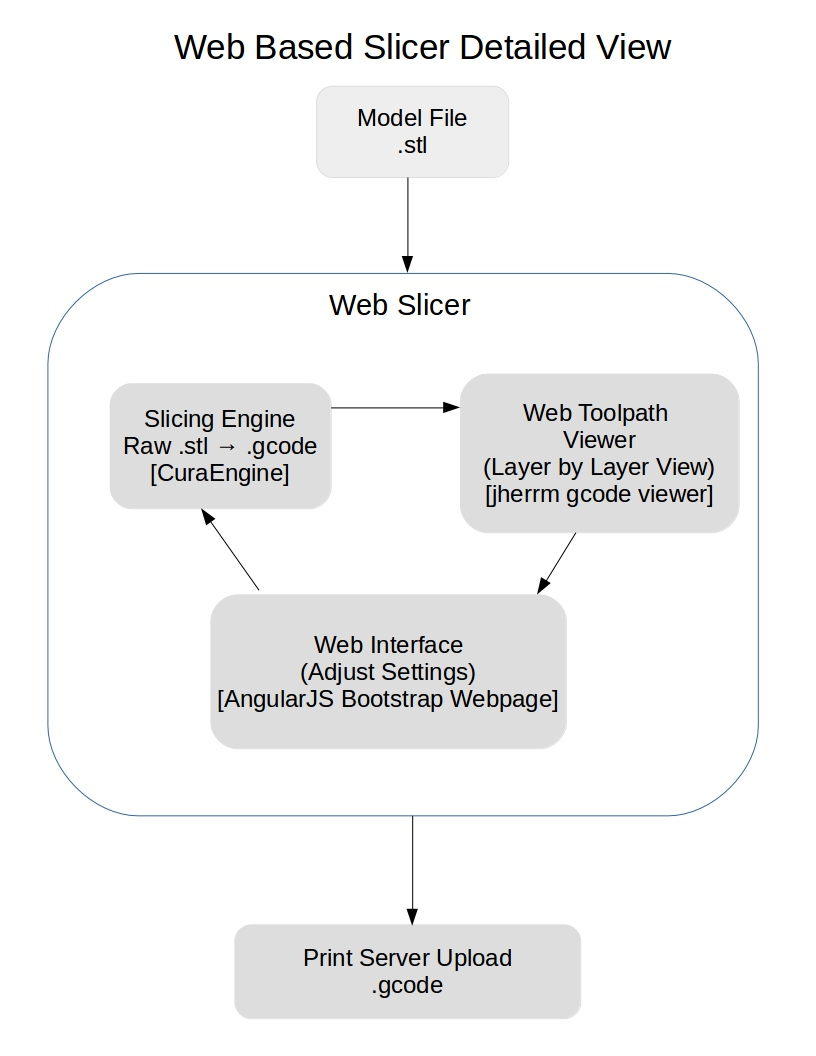
\includegraphics[width=\linewidth]{slicer-detailed-view}
  \caption{High level view of how WebSlicer functions and how users will interact with it}
  \label{fig:slicer-detailed-view}
\end{figure}

\section{Working procedure}
\paragraph{}
As shown in Figure \ref{fig:slicer-detailed-view}, the application will have 3 major components that all need to work together in a cycle until the user decides that the output is what they desire.

\subsection{Web Interface}
\paragraph{}
I anticipate that it will include a set of forms for collecting the users settings for their printer and account tracking info so that they may retain certain settings. 
Additionally, I would like to include a gcode editor which will allow users to edit specific portions of their gcode and see the resulting output in the viewer. 
This does not include the actual slicing engine which must be driven and accessed independently.

\subsection{Slicing Engine}
\paragraph{}
The slicing engine is at the heart of this project. 
It will include taking uploaded .stl model files by the user and convert them into raw G-code. 
The engine that carries out the raw geometry calculations is CuraEngine and is written in pure C++, (it is not web friendly). 
Thus, this portion of the project will require deploying CuraEngine at a cloud provider and then creating a RESTful API to interface with it.

\subsection{Web Tool Path Viewer}
\paragraph{}
After configuring and generating the G-code representation for a 3D model, there still must be a way to review visually how the slicing engine actually will split up the model. 

\subsection{Final Steps}
\paragraph{}
The final step in the process of this application will be creating links to the finished files where the user can either choose to download the completed G-code file. 
If the user has access to a print server such as OctoPrint, they may opt to copy/paste the link to it where it will be uploaded automatically for printing using the OctoPrint API.

\section{Review and Usability Testing}
\paragraph{}
After running throguh all steps of the working procedure running through a round of usability testing was pertinant as no good design should go unreviewed.
